\section{Introduction}


In recent years, the barriers to the development of Artificial Intelligence (AI) have been broken down with the rapid progress of ABC technologies in computing: AI, Big Data, and Cloud Computing, as well as the emergence of cost-effective specialized hardware~\cite{sze2017efficient} and software~\cite{jia2014caffe}. This has led to the world entering the third wave of AI development: Deep Learning~\cite{lecun2015deep}.
The success of current data-driven AI relies on massive amounts of training data and follows a gather-and-analyze paradigm~\cite{whang2023data}, which confronts with challenges of complying with rigorous data protection regulations such as OECD Privacy Guidelines~\cite{tene2011privacy} and General and Data Protection Regulation (GDPR)~\cite{voigt2017eu}.
%So although data-centric AI is now the mainstream, a novel model-centric distributed collaborative training framework called Federated Learning is gaining popularity in both academia and industry due to its advantages in complying with privacy regulations.
So although data-centric AI is currently mainstream paradigm, Federated Learning~\cite{li2020federated}, a novel model-centric distributed collaborative training framework, is gaining popularity in both academia and industry for its advantages in complying with privacy regulations~\cite{truong2021privacy}.

According to the definitions of IEEE Standard for Federated Machine Learning (FML, aka FL)~\cite{IEEEstd3652}, \textit{FL is a framework or system that enables multiple participants to collaboratively build and use machine learning models without disclosing the raw and private data owned by the participants while achieving good performance.}
For example, a typical workflow of FL systems is that the entity with modeling demand (aka FL server) first deploys the FL services and initializes the model training task, and then distributing this task  to participants with training data (aka FL clients) for modeling~\cite{bonawitz2019towards}.
Based on this workflow pattern, many FL frameworks have been derived with specialized improvements in communication~\cite{konevcny2016federated, mcmahan2017communication, xu2021asynchronous}, optimizaiton~\cite{li2018federated, karimireddy2020scaffold, li2021model}, robustness~\cite{duan2020self, sattler2019robust, li2022federated} and privacy~\cite{bonawitz2017practical, geyer2017differentially, cheng2021secureboost}.
While these fascinating improvements greatly enhance the utility of FL, they all follow a task-based interaction paradigm, in which an FL server dominates the cooperation between FL participants.
In this narrow interpretation of FL, the data owner is treated more like a worker than a collaborator and performs training primarily for the benefit of the server's goals.
Due to the above defects, clients have little enthusiasm to participate, and the potential for redundant training also leads to low model reusability, further diminishing the efficiency of the FL systems.
This explains why current FL frameworks are more akin to private distributed modeling services rather than sustainable and privacy-preserving modeling platforms for everyone as expected.

\begin{figure}[b]
    \centering
    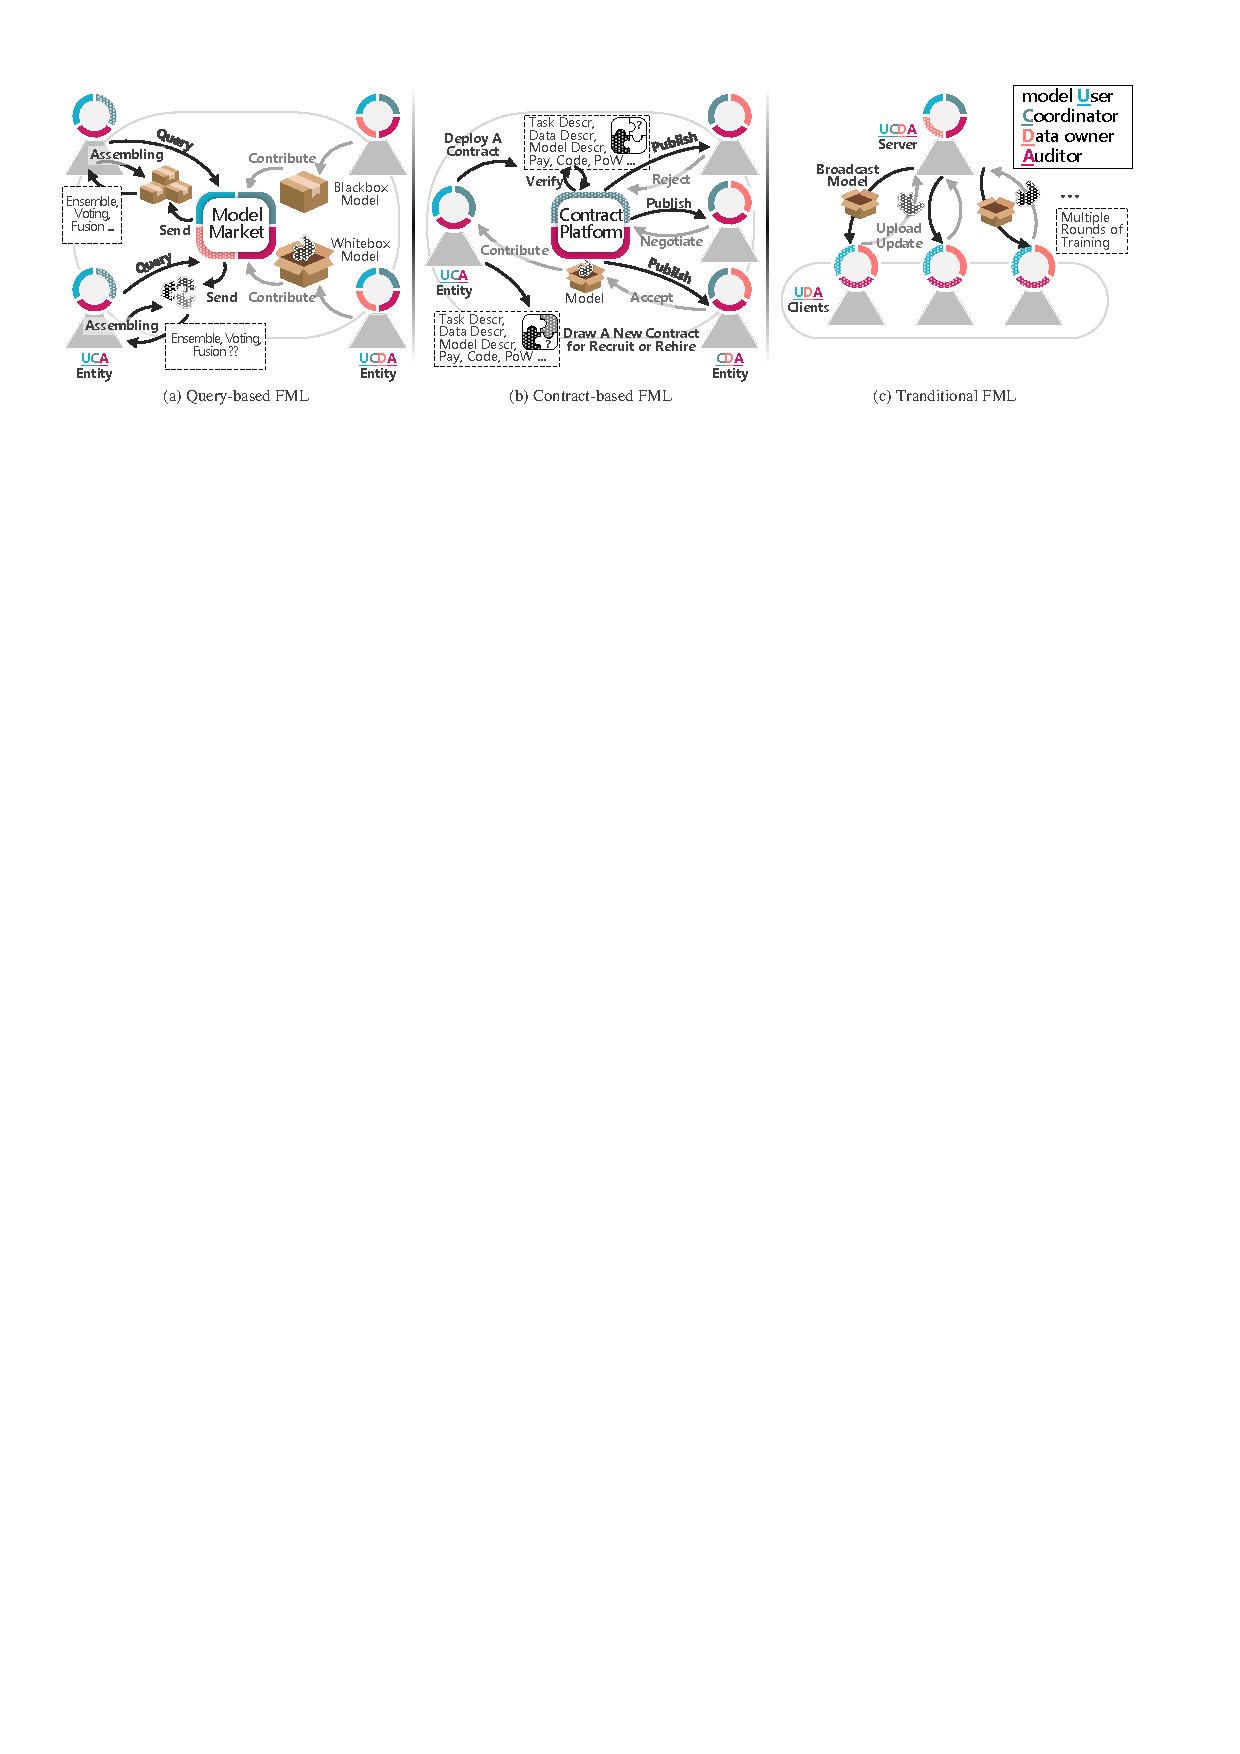
\includegraphics[width=\linewidth]{fig/coop_frame.pdf}
    \caption{A schematic diagram of three cooperation frameworks of FL. (a) (b) are the proposed open FL platforms, (c) is the traditional FL platform. Four colors correspond to four roles in~\cite{IEEEstd3652}, and colors with grid lines indicate non-essential roles.}
    \Description{}
    \label{fig:coop}
\end{figure}

In this paper, we try to answer the question: \textbf{Can we establish a sustainable open FL platform based on a novel reciprocal cooperation framework?}
Obviously, to answer this quesion, it is insufficient simply study the basic concepts of FL and investigate existing FL techniques.
We also need to conduct a wide survey of potential techniques that can facilitate the construction of open FL platforms.
To aid understanding, Fig.~\ref{fig:coop} provides a first glimpse of two novel FL cooperation frameworks we advocated: 
\begin{itemize}
    \item \textbf{Query-based FL.} It follows a loosely-coupled cooperation framework between entities (we use "entities" instead of "participants" to emphasizes equality), where any entity can freely upload their local models or retrieve models from an open repository named Model Community.
    There are many valuable challenges that can be explored, such as how to query for models, how to reuse the retrieved models or how to transfer knowledge from these models, how to ensure the legal compliance between different model licenses, how to protect the intelligent properties of released models (ref. Section~\ref{sec:query}). %TODO: 
    \item \textbf{Contract-based FL.} It follows a mutual choice cooperation framework, where each entity can deploy model training contracts with specialized requirements such as task modality, execution environment, model architecture and license. Meanwhile, entities holding data can choose whether to accept the contract.
    Research topics in this setting include model pricing, model ownership verification and .... (ref. Section~\ref{}) % TODO:
\end{itemize}
It's worth noting that the definitions of the four roles illustrated in Fig.~\ref{fig:coop} (i.e. model user, coordinator, data owner, auditor, ref. Section~\ref{sec:basicdefinition}) are adopted for compatibility with the IEEE standard~\cite{IEEEstd3652}, and our proposals are also within the standard definitions of FML.
The diagram in Fig.~\ref{fig:coop}(c) illustrates the workflow of traditional FL, where all FL clients are required to accept the training schedule from the FL server and perform multiple rounds of local training and model averaging until the global model converges.
In contrast, the entities in query-based FL and contract-based FL are proactive in their participate.
We believe that these reciprocal cooperation frameworks have the potential to expand the prevalence of open FL and establish FL ecosystems.


\subsection{Our Contribution}
  In contrast to previous surveys that primarily focused on the server-dominated cooperation framework in FL,  our new survey explores the feasibility of reciprocal cooperation frameworks in FL.
  To the best of our knowledge, our work represents the first systematic survey in this area.
  The major contributions of this survey are as follows:
  \begin{itemize}
      \item We introduce the concept of open FL platforms by presenting two reciprocal cooperation frameworks, namely query-based FL and contract-based FL, along with an overview of their key features and properties.
      \item We explore the query functionalities of online model repositories, such as Huggingface and OpenVINO, to investigate their feasibility for model query in query-based FL settings.
      \item We summarize the rights, restrictions, and enforcements of in-service model licenses and highlight the legal compliance and copyrightability issues in collaborative modeling. Additionally, we provide guidelines for selecting licenses to minimize conflicts and prevent license proliferation.
      \item We propose a new taxonomy to streamline the legal compliance analysis in FL studies, which is also useful for quickly identifying suitable model reusing methods for open FL platforms. A comprehensive comparison of current FL studies based on this taxonomy is surveyed.
      \item We analyze the requirements for model protection in the context of query-based FL and identify applicable solutions from deep intellectual property protection technologies.
\end{itemize}
  
The rest of this paper is organized as follows. 
We compare this survey to other related surveys and show our distinction in Section~\ref{sec:related}. 
In Section~\ref{sec:basic}, we presente the overview and point the limitations of traditional FL.
We comprehensively explore the feasibility and challenges of query-based FL in Section~\ref{sec:query}, which includes model query (Section~\ref{sec:how2query}), model license comparison (Section~\ref{sec:licensing}) and selection (Section~\ref{sec:choosing}), copyright issues (Section~\ref{sec:generated content}), and analysis of license conflicts in model reusing (Section~\ref{sec:reusing&license}).
In Section~\ref{sec:taxonomy}, we present our taxonomy from a model reusing perspective, and in Section~\ref{sec:hybrid}, we summarize FL studies based on this new taxonomy.
The discussion on model protection is presented in Section~\ref{sec:how2protect}.


%By investigating reciprocal cooperation frameworks, we aim to broaden the understanding of FL and uncover new opportunities for collaboration and data sharing among participants. Through our comprehensive analysis, we provide valuable insights and recommendations for researchers and practitioners interested in exploring and implementing reciprocal cooperation in FL settings.
